\documentclass[10pt,oneside,final,notitlepage,a4paper,wide]{mwart} 
\usepackage[utf8]{inputenc} 
\usepackage{polski} 
\usepackage{graphicx}
\usepackage{setspace}

\onehalfspacing
\setlength{\parindent}{0cm} 

\usepackage[]{hyperref}
\usepackage{hyperref,xcolor}% http://ctan.org/pkg/{hyperref,xcolor}
\usepackage{makeidx}

\definecolor{orangelink}{rgb}{0.7,0.18,0.1} 

\hypersetup{
    pdftitle={Alleluia Pasquale - Dominica Paschæ in Resurrectione Domini - Ad Vigiliam Paschalem in Nocte Santa},
    pdfdisplaydoctitle=true,
    pdfauthor={pitrk, JanekR_Prorok},
    pdfsubject={Source: https://github.com/JanekRProrok/Triduum_Sacrum},
    pdfcreator={Texmaker, MiKTeX},
    pdfproducer={},
    pdfinfo={},
    pdfkeywords={},
    bookmarks=true,
    bookmarksnumbered=true,
    bookmarksopen=true,
    bookmarksopenlevel=1,
    pdfpagelabels=true,
    pdfpagemode=UseOutlines,
    unicode=true,
    pdftoolbar=true,
    pdfmenubar=true,
    pdffitwindow=false,
    pdfstartview=Fit,
    pdfnewwindow=true,
    colorlinks=true,
    linkcolor=orangelink,
    citecolor=orangelink,
    filecolor=orangelink,
    urlcolor=orangelink,
    pdfpagelayout=TwoPageRight,
}
% http://www.tug.org/applications/hyperref/manual.html#x1-120003.8

%------------------------------------------------------------------------------%
%------------------------------------------------------------------------------%

	% Wypełnienie ... \dotline{długość+0,1cm}.
\def\dotfill#1{\cleaders\hbox to #1{.}\hfill}
\newcommand\dotline[2][0,1cm]{\leavevmode\hbox to #2{\dotfill{#1}\hfil}}	
	
%------------------------------------------------------------------------------%

\begin{document}
% \sloppy - Wymuszenie nieprofesjonalnego trzymania się w marginesach (kosztem dziwnie rozciągniętych odstępów).
%
\begin{center}
	\LARGE{\textbf{Dominica Paschæ in Resurrectione Domini\\Ad Vigiliam Paschalem in Nocte Santa\\Alleluia Pasquale}}\\ \smallskip
	\small{Niedziela Zmartwychwstania Pańskiego\\Wigilia Paschalna w Wielką Noc\\Alleluja Paschalne\\ \smallskip Stacja u Św. Jana na Lateranie}
\vspace{1cm}

	\begin{figure}[h]
		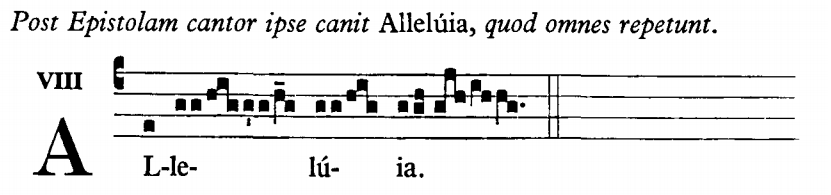
\includegraphics[width=\textwidth]{Alleluia_Choral.png}
	\end{figure}
	\large{Śpiew Alleluja jest powtarzany trzykrotnie,\\za każdym razem zaczynając od wyższego dźwięku.}
	\begin{figure}[h]
		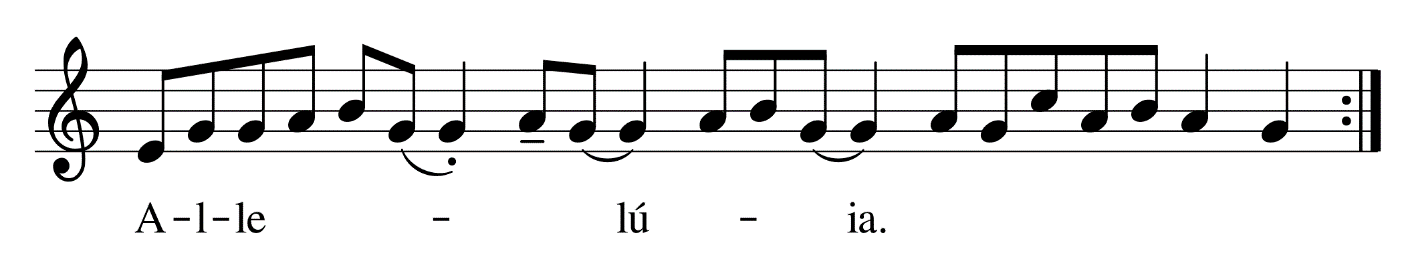
\includegraphics{Alleluia_notes.png}
	\end{figure}
\end{center}
\bigskip

Przykładowe wykonania:
	\begin{itemize}
		\item Watykan 2011 -- \href{https://youtu.be/4DvRrrdOfbo}{https://youtu.be/4DvRrrdOfbo}
		\item Watykan 2013 -- \href{https://youtu.be/k89SA3lBdKI}{https://youtu.be/k89SA3lBdKI}
		\item Frombork 2015 -- \href{https://youtu.be/kpDhlek1h0w}{https://youtu.be/kpDhlek1h0w}
		\item Pogórze 2018 -- \href{https://youtu.be/MJ4hgMCgcRI}{https://youtu.be/MJ4hgMCgcRI}
	\end{itemize}
\end{document}